\chapter{Implementation}
\label{cha:implementation}

This chapter will provide an overview over Whisker's implementation.
Because Whisker is still in early development, some of its implementation may change later.

\section{Implementation Environment}
\label{sec:implementation_environment}

Whisker uses Scratch 3.0, which is implemented in JavaScript.
Therefore, it is also implemented in JavaScript (ES6) for compatibility.
One restriction of Whisker's implementation environment is Scratch's dependence on a renderer.
In order to operate properly, the Scratch VM needs a HTML canvas to render to.
This limits Scratch, and consequently Whisker, to run inside a web environment.
Therefore, we use webpack\footnote{\url{https://webpack.js.org/}} to transpile Whisker's source code into browser-runnable JavaScript.

\section{General Architecture}
\label{sec:general_architecture}

One of Whisker's main design goals is to leave the Scratch virtual machine unchanged.
There are two reasons for this decision.
For one thing, if Whisker used a modified version of Scratch,
the modified version would need to be updated regularly as the original version of Scratch receives updates.
But the main reason for this decision is that it allows Whisker to be attached to any instance of the Scratch VM.
Therefore, anything that runs Scratch 3.0 can theoretically use Whisker.
\parspace

Figure~\ref{fig:general_architecture} shows Whisker's general architecture.
It is designed to be a layer between test code and the Scratch virtual machine.
The main class \texttt{VMWrapper} makes up a wrapper around the Scratch virtual machine,
and its components each implement one part of Whisker's functionality.
Test code uses a test driver object, which gives access to the methods that are used for testing.
The test driver is used instead of directly interacting with the VM wrapper,
because it offers a simpler interface and prevents access to Whisker's private methods.
\parspace

\begin{figure}[htpb]
    \centering
    \tikzset{>=latex,
             arrow/.style={-{Latex[length=1.5mm, width=1.5mm]}},
             label/.style={draw=none, text width=5.3cm, minimum height=0.5cm, text centered},
               box/.style={draw,      text width=3.2cm, minimum height=0.7cm, text centered, rounded corners},
                 h/.style={fill=blue!10}}

    \begin{tikzpicture}
        \node[box]   at ( 0.00,  3.0) (testcode)      {Test Code};
        \node[box]   at ( 0.00,  1.5) (testdriver)    {Test Driver};
        \node[label] at ( 0.00,  0.0) (vmwrapper)     {\textbf{VM Wrapper}};
        \node[box]   at (-1.80, -0.7) (inputs)        {Inputs};
        \node[box]   at ( 1.85, -0.7) (random-inputs) {Random Inputs};
        \node[box]   at (-1.80, -1.6) (sprites)       {Sprites};
        \node[box]   at ( 1.85, -1.6) (callbacks)     {Callbacks};
        \node[box]   at (-1.80, -2.5) (constraints)   {Constraints};
        \node[box]   at (-2.00, -4.1) (scratchvm)     {Scratch VM};
        \node[box]   at ( 2.20, -4.1) (scratchrender) {Scratch Renderer};
        \node[box]   at (-2.00, -5.8) (otherscratch)  {Other Scratch Components};

        \begin{scope}[on background layer]
            \node[draw, h, rounded corners, fit=(vmwrapper)(sprites)(inputs)(callbacks)(constraints)(random-inputs)] (container) {};
        \end{scope}

        \foreach \pp/\pf/\pt in {--/testcode/testdriver,
                                 --/testdriver/container,
                                 --/container/scratchvm,
                                 --/container/scratchrender,
                                 --/scratchvm/scratchrender,
                                 --/scratchvm/otherscratch}
            \draw[shorten >= 2pt, arrow] (\pf) \pp (\pt);

        % \draw[shorten >= 2pt, rounded corners, dashed, ->]
        %        (constraints)
        %     -- ( 3.5, -1.6)
        %     -- ( 3.5,  3.0)
        %     -- (testcode);
        % \draw[dashed, -] (callbacks) -- ( 3.5, -0.7);
    \end{tikzpicture}

    \caption{General architecture of Whisker}
    \label{fig:general_architecture}
\end{figure}

\section{Scratch Program Execution and the Step Loop}
\label{sec:scratch_program_execution_and_the_step_loop}

The core of Scratch's virtual machine is a function called \texttt{step},
which is called at a constant frequency of 30 times per second using JavaScripts \texttt{setInterval} mechanism.
It runs the program until a time limit is reached, then it draws the scene using the renderer.
If some visual change occurs, i.e.\ when a sprite changes appearance or position, a redraw is requested,
and the program execution step is stopped earlier (in turbo mode redraw requests are ignored).
Figure~\ref{lst:simplified_scratch_step} shows a simplified version of this procedure.
\parspace

\begin{listing}[htpb]
    \centering
    \begin{subfigure}{.9\textwidth}
        \begin{javascriptcode}
            _step () {
                this.threads = this.threads.filter(thread => !thread.isKilled);

                /* Execute the active scripts. */
                this.sequencer.stepThreads();

                /* Render if a renderer is attached. */
                if (this.renderer) {
                    this.renderer.draw();
                }

                /* Emit events. */
                ...
            }

            start () {
                /* Execute the step function 30 times per second. */
                this._steppingInterval = setInterval(() => {
                    this._step();
                }, THREAD_STEP_INTERVAL);
            }
        \end{javascriptcode}
        \vspace{-\bigskipamount}
        \caption{Simplified \texttt{step} and \texttt{start} functions from Scratch's \texttt{Runtime} class}
    \end{subfigure}

    \bigskip

    \begin{subfigure}{.9\textwidth}
        \begin{javascriptcode}
            stepThreads () {
                WORK_TIME = 0.75 * THREAD_STEP_INTERVAL;
                this.timer.start();

                /* Execute the program until there is no more work,
                 * the work time is up, or a redraw is requested. */
                while (numActiveThreads > 0 &&
                       timer.timeElapsed() < WORK_TIME &&
                       (!this.runtime.redrawRequested || this.runtime.turboMode)) {

                    /* Execute each script sequentially. */
                    for (thread of this.runtime.threads) {
                        /* Execute the thread until either the script's end
                           is reached, one loop iteration is executed,
                           or the thread yields. */
                        this.stepThread(thread);
                    }
                }
            }
        \end{javascriptcode}
        \vspace{-\bigskipamount}
        \caption{Simplified \texttt{stepThreads} function from Scratch's \texttt{Sequencer} class}
    \end{subfigure}
    \caption{Simplified Scratch step code}
    \label{lst:simplified_scratch_step}
\end{listing}

For the purpose of controlling the execution of the program, and to run multiple functions alongside the step loop,
Whisker clears the interval that runs the \texttt{step} function and runs its own loop, which in turn calls Scratch's \texttt{step} function, instead.
Figure~\ref{fig:whisker_step_procedure} shows the procedure of Whisker's step function.
In addition to running the Scratch program, it performs other tasks which have to be executed periodically.%
\parspace

\begin{figure}[htpb]
    \centering

    \tikzset{>=latex,
           arrow/.style={draw, -{Latex[length=1.5mm, width=1.5mm]}},
             box/.style={draw, text width=4.5cm, minimum height=0.7cm, text centered, rounded corners},
             num/.style={draw, circle, inner sep=0.6mm, text centered},
               h/.style={fill=blue!10}}

     \begin{tikzpicture}
        \node[box]    at ( 0.2,  5.0) (callbacksbefore) {Call Callbacks (before)};
        \node[box]    at ( 0.2,  4.0) (random-inputs)   {Perform Random Inputs};
        \node[box]    at ( 0.2,  3.0) (inputs)          {Perform Inputs};
        \node[box]    at ( 0.2,  2.0) (sprites)         {Update Sprites};
        \node[box, h] at ( 0.2,  1.0) (step)            {Step Scratch Program};
        \node[box]    at ( 0.2,  0.0) (callbacksafter)  {Call Callbacks (after)};
        \node[box]    at ( 0.2, -1.0) (constraints)     {Check Constraints};

        \node[num] at (-2.6,  5.0) (one)   {1};
        \node[num] at (-2.6,  4.0) (two)   {2};
        \node[num] at (-2.6,  3.0) (three) {3};
        \node[num] at (-2.6,  2.0) (four)  {4};
        \node[num] at (-2.6,  1.0) (five)  {5};
        \node[num] at (-2.6,  0.0) (six)   {6};
        \node[num] at (-2.6, -1.0) (seven) {7};

        \draw[shorten >= 2pt, rounded corners, arrow]
               ( 0.2,  6.0)
            -- (callbacksbefore)
            -- (random-inputs)
            -- (inputs)
            -- (sprites)
            -- (step)
            -- (callbacksafter)
            -- (constraints)
            -- ( 0.2, -2.0);
    \end{tikzpicture}

    \caption{Whisker's step procedure}
    \label{fig:whisker_step_procedure}
\end{figure}

To make running and pausing the program on demand possible, we implemented a class called \texttt{Stepper},
which queues and periodically executes functions in a fixed frequency using JavaScript's intervals as needed.
Whenever a test runs the Scratch program,
the \texttt{Stepper} is used to execute Whisker's own \texttt{step} function periodically,
until the execution is done.
Listing~\ref{lst:run_method_excerpt} shows an excerpt of Whisker's run method,
in which the step loop is implemented.
Although the Scratch program has to be run asynchronously, we use JavaScript's \texttt{Promise} API to make running the program seem like a normal method call.
Tests are declared as \texttt{async functions}, so they can use the \texttt{await} keyword to wait until a run of the program is done.
Otherwise, other test code would continue to be executed while the JavaScript engine waits for the next Scratch step.
Figure~\ref{lst:promise_api_example} presents a code example for this.
Whisker prevents multiple runs of the Scratch program at the same time by throwing an error,
when a run of the program is being started, while another one is still going on.
\parspace

\begin{listing}[htpb]
    \centering

    \begin{minipage}{.9\textwidth}
        \begin{javascriptcode}
            async run (condition, timeout, steps) {
                ...
                while (this.running &&
                       this.getRunTimeElapsed() < timeout &&
                       this.getRunStepsExecuted() < steps &&
                       !condition()) {
                    await this.stepper.step(this.step.bind(this));
                    ...
                }
                ...
            }
        \end{javascriptcode}
    \end{minipage}

    \caption{Excerpt from Whisker's run method}
    \label{lst:run_method_excerpt}
\end{listing}

\begin{listing}[htpb]
    \centering

    \begin{minipage}{.9\textwidth}
        \begin{javascriptcode}
            const test = async function (t) {
                await t.runForTime(1000);
                console.log('This will be executed after the run ends.');

                t.runForTime(1000);
                console.log('But this will be executed during the run (no await).');
            }
        \end{javascriptcode}
    \end{minipage}

    \caption{Using JavaScript's Promise API to wait for runs}
    \label{lst:promise_api_example}
\end{listing}

Running other code before and after Scratch's step could theoretically be problematic in a single-threaded environment like JavaScript,
because it could take longer than the allowed 1/30 second per step and therefore slow down the Scratch program.
But in reality, most Scratch programs will only use a fraction of the allocated work time for the step,
because they visually change sprites in every step, which makes the step finish earlier due to the issued redraw request.
And even when no redraw is requested,
the allocated time interval for rendering the picture is long enough to allow Whisker to run its other tasks without exceeding the time limit of 1/30 second.
Therefore, Whisker can run other tasks in between the Scratch steps without interfering with the program.
In section~\ref{sec:rq3}, we will prove this empirically by measuring how long Scratch's steps and Whisker's other tasks take to execute.

\section{Accessing Sprites and Variables}
\label{sec:accessing_sprites_and_variables}

Scratch's implementation differentiates between \texttt{Sprites} and \texttt{RenderedTargets}.
\texttt{Sprite} objects contain the scripts, costumes, and sounds of the sprite.
They can be seen as a kind of blueprint for the actual sprite instances, which are objects of the \texttt{RenderedTarget} class.
In contrast, we will call rendered targets sprites, since this resembles the user's view.
\parspace

Whisker implements a wrapper class around \texttt{RenderedTarget}
and provides access to these wrappers, instead of the sprite objects themselves.
This serves two purposes:
Firstly, the wrapper objects offer a simpler and more test-friendly interface.
This interface allows to access the sprite's attributes (i.e. the attributes of the \texttt{Sprite} object and the \texttt{RenderedTarget} object),
provides useful helper methods for testing,
and gives access to the sprite's variables.
Secondly, it saves the sprite's attributes and variable values from the last rendered frame,
which is very useful for testing.
These attributes are made available in the \texttt{old} attribute of the sprite wrapper.
The \texttt{old} values are updated, i.e. replaced with the current values,
before every step of the Scratch program.
This is illustrated in Whisker's step procedure shown by Figure~\ref{fig:whisker_step_procedure} in step 4.
\parspace

In order to keep track of the sprite wrappers,
Whisker keeps a mapping between the unique id of the original \texttt{RenderedTarget} objects and their wrappers.
Whenever a sprite is requested, Whisker first checks the mapping for an existing wrapper,
and only creates a new one if there isn't already one for the specific sprite.
This way, only one wrapper object can exist for every sprite in the program.
The same thing is done with variables.
Each sprite wrapper keeps track of its own variables.

\section{Simulating Inputs}
\label{sec:simulating_inputs}

Scratch's virtual machine provides an interface to perform input events on the Scratch program through its \texttt{postIOData} method.
This method is usually used by Scratch's GUI, which forwards input events from the web browser to the virtual machine.
But we can use this API for Whisker to simulate mouse and keyboard inputs.
However, \texttt{postIOData} is not a very user-friendly interface,
as it requires extra information about the Scratch stage and coordinate conversion for mouse inputs.
Because of this, Whisker takes inputs in a slightly simpler format and converts them to the format that \texttt{postIOData} expects.
Listing~\ref{fig:input_conversion_example} shows a mouse input in Whisker's format and the resulting \texttt{postIOData} call.
Answers to Scratch's \texttt{ask} blocks, are simulated in a similar way, but though the VM's event system instead of \texttt{postIOData}.
\parspace

\begin{listing}[htpb]
    \centering

    \begin{subfigure}[b]{.25\textwidth}
        \begin{javascriptcode}
            t.inputImmediate({
                device: 'mouse',
                isDown: true,
                x: 50,
                y: 100
            });
        \end{javascriptcode}
        \vspace{-\bigskipamount}
        \caption{A mouse input in Whisker's format}
    \end{subfigure}
    \hspace{.08\textwidth}
    \begin{subfigure}[b]{.3\textwidth}
        \begin{javascriptcode}
            vm.postIOData('mouse', {
                isDown: true,
                x: 194.09,
                y: 53.65,
                canvasWidth: 321.25,
                canvasHeight: 241.43
            });
        \end{javascriptcode}
        \vspace{-\bigskipamount}
        \caption{The resulting \texttt{postIOData} call}
    \end{subfigure}

    \caption{Resulting IO event from a mouse input}
    \label{fig:input_conversion_example}
\end{listing}

Whisker provides methods to either perform inputs immediately,
or to queue inputs and execute them after a certain time has passed during the next run of the program.
For this purpose, Whisker keeps a list of inputs, which are supposed to be performed later.
When the program under test is executed, these inputs are checked before every Scratch step
and inputs, which are due, are performed.
Figure~\ref{fig:whisker_step_procedure} illustrates when the inputs are called in Whisker's step procedure.
\parspace

Some inputs encompass multiple IO events.
For example, pressing a key for a certain duration and then releasing it requires two input events.
For this purpose, Whisker keeps a state for each input,
which indicates how much of the input was already performed,
and what action has to be carried out next.

\section{Automated Input Generation}
\label{sec:automated_input_generation}

We implemented a simple form of automated input generation using of Whisker's randomized inputs.
The algorithm detects which inputs the program under test responds to,
and registers random inputs accordingly.
To determine the inputs, Whisker simply iterates through the blocks of the currently loaded program
and searches for certain block types and block configurations, which detect user inputs.
Then it registers a random input for each found configuration.
\parspace

Table~\ref{tab:scratch_input_blocks} lists block configurations, which depend on user inputs,
and the resulting inputs, which get registered for each block configuration.
Each resulting input depends only on the block type and its parameter.
The only exception to this are inputs that answer seeded strings to \texttt{ask} blocks.
Whisker checks for comparisons between the \texttt{answer} variable and string constants.
These string constants are then seeded as possible answers for the \texttt{ask} blocks.
\parspace

\newcommand{\tablebox}[1]{
    \begin{tikzpicture}
         \node[draw, text width=8.5cm, minimum height=0.6cm, rounded corners] {\footnotesize #1};
    \end{tikzpicture}
}

\begin{table}[htpb]
    \centering

    \renewcommand{\baselinestretch}{0.8}

    \scalebox{0.875}{
        \begin{tabular}{m{5.25cm}m{9.0cm}}
            \toprule
            Scratch Block(s) & Resulting Input(s) \\
            \midrule
            \vspace{3.5mm}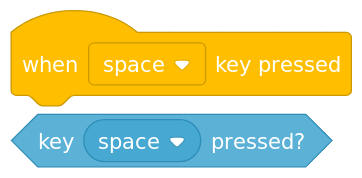
\includegraphics[scale=1.5]{scratch-input-blocks-1}\vspace{2mm} & \tablebox{(1) Press the respective keyboard key}                \\
            \vspace{3.5mm}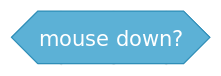
\includegraphics[scale=1.5]{scratch-input-blocks-2}\vspace{2mm} & \tablebox{(1) Click the left mouse button}                      \\
            \vspace{3.5mm}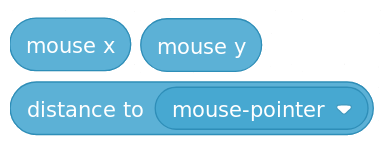
\includegraphics[scale=1.5]{scratch-input-blocks-3}\vspace{2mm} & \tablebox{(1) Move the cursor to a random position}             \\
            \vspace{3.5mm}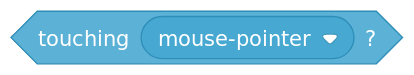
\includegraphics[scale=1.5]{scratch-input-blocks-4}\vspace{2mm} & \tablebox{(1) Move the cursor near / onto the respective sprite \\
                                                                                                      (2) Move the cursor to a random position}             \\
            \vspace{3.5mm}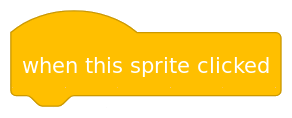
\includegraphics[scale=1.5]{scratch-input-blocks-5}\vspace{2mm} & \tablebox{(1) Click near / onto the respective sprite           \\
                                                                                                      (2) Click on a random position}                       \\
            \vspace{3.5mm}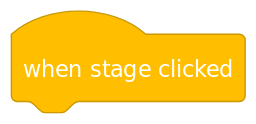
\includegraphics[scale=1.5]{scratch-input-blocks-6}\vspace{2mm} & \tablebox{(1) Click on a random position}                       \\
            \vspace{3.5mm}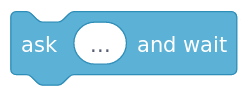
\includegraphics[scale=1.5]{scratch-input-blocks-7}\vspace{2mm} & \tablebox{(1) Answer with a randomly generated string}          \\
            \vspace{3.5mm}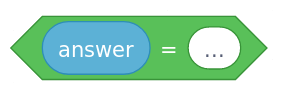
\includegraphics[scale=1.5]{scratch-input-blocks-8}\vspace{2mm} & \tablebox{(1) Answer with the compared string constant}         \\
            \bottomrule
        \end{tabular}
    }

    \caption{Scratch's input blocks and their resulting generated inputs}
    \label{tab:scratch_input_blocks}

    \renewcommand{\baselinestretch}{\oldbls}
\end{table}

\section{Callbacks and Constraints}
\label{sec:callbacks_and_constraints}

Callbacks and constraints are both implemented as JavaScript functions,
that are periodically called during the program execution.
When they are registered, they are simply put into a list.
Then, during the step procedure,
Whisker iterates over both lists and executes every callback and constraint.
Both callbacks and constraints can be enabled and disabled,
which adds or removes them from their respective list.
\parspace

Constraints have one key difference to normal callbacks.
When constraints are executed, assertion errors are caught.
When an error is caught, the constraint is removed from the list,
and the error is forwarded to the VM wrapper.
This makes it possible to react to failed constraints in different ways.
The VM wrapper can, depending on configuration, re-throw the error to fail the test,
stop the current run of the program,
or ignore the constraint failure entirely.

\section{Coverage Measurement}
\label{sec:coverage_measurement}

Whisker can be used to measure statement coverage on Scratch programs.
It does this by temporarily modifying Scratch's \texttt{Thread} class.
This class has two methods, \texttt{pushStack} and \texttt{reuseStackForNextBlock},
which put blocks onto the execution stack.
Whisker intercepts these methods by replacing them with a version
that saves the unique id of the executed blocks and then calls the respective original method.
This way, Whisker can track which blocks are executed by the program.
\parspace

In order to calculate the coverage, we also need a complete list of the program's blocks.
To compose this list, Whisker traverses all scripts of the program
and saves each block's unique id.
Because Whisker traverses the scripts, blocks which are not part of a script with a hat
are ignored for the coverage measurement.
This is not a problem, since these blocks are not reachable by the program anyways.
Whisker considers all reachable control structure blocks, statement blocks and hats for the statement coverage.
Coverage is measured per sprite, and program wide coverage can simply be calculated from the per-sprite coverage.
Listing~\ref{fig:example_coverage_report} shows an example coverage report and
Listing~\ref{fig:measuring_coverage} gives a code example of how to measure statement coverage with Whisker.
\parspace

\begin{listing}[htpb]
    \centering

    \begin{minipage}{.5\textwidth}
        \begin{javascriptcode}
              { stage: { covered: 0, total: 0 },
                bowl: { covered: 16, total: 16 },
                bananas: { covered: 12, total: 24 },
                apple: { covered: 15, total: 18 } }
        \end{javascriptcode}
    \end{minipage}

    \caption{Example coverage report}
    \label{fig:example_coverage_report}
\end{listing}

Currently, coverage measurement can only be performed on Scratch 3.0 (.sb3) projects,
since earlier projects don't make the unique id of each block persistent in the project file.
However, this is not a problem since older Scratch projects can simply be converted to Scratch 3.0 projects by
opening them in Scratch 3.0 and saving them.
\parspace

\begin{listing}[htpb]
    \centering

    \begin{minipage}{.75\textwidth}
        \begin{javascriptcode}
            /* (1) Replace pushStack and reuseStackForNextBlock,
               so the executed blocks can be tracked. */
            CoverageGenerator.prepareThread(Thread);

            /* (2) Traverse the scripts of the currently loaded program
               and gather a list of all reachable blocks. */
            CoverageGenerator.prepare(vm);

            /* Run the Scratch program.
            * (Can be run and reloaded multiple times.) */
            ...

            /* (3) Retrieve the current statement coverage. */
            const coverage = CoverageGenerator.getCoverage();

            /* (4) Restore the original implementations of pushStack and
               reuseStackForNextBlock. */
            CoverageGenerator.restoreThread(Thread);
        \end{javascriptcode}
    \end{minipage}

    \caption{Example code for coverage measurement using Whisker}
    \label{fig:measuring_coverage}
\end{listing}

In order to measure coverage, one has to gain access to Scratch's \texttt{Thread} class.
This can be achieved either at compile time or at runtime.
Listing~\ref{fig:acquiring_thread_class} shows example code of how this can be done.
\parspace

\begin{listing}[htpb]
    \centering

    \begin{subfigure}[b]{.7\textwidth}
        \begin{javascriptcode}
            const VirtualMachine = require('scratch-vm');
            const Thread = require('scratch-vm/src/engine/thread');
        \end{javascriptcode}
        \vspace{-\bigskipamount}
        \caption{At compile time using JavaScript's module system}
    \end{subfigure}

    \bigskip

    \begin{subfigure}[b]{.7\textwidth}
        \begin{javascriptcode}
            const Thread = vm.runtime.threads[0].__proto__
        \end{javascriptcode}
        \vspace{-\bigskipamount}
        \caption{At runtime by getting the class of a running \texttt{Thread} instance}
    \end{subfigure}

    \caption{Acquiring Scratch's Thread class}
    \label{fig:acquiring_thread_class}
\end{listing}
